\subsection{Гипербола}

\newcommand{\term}[1]{{\sffamily #1}}
 
\textit{Гипербола} --- геометрическое место точек евклидовой плоскости, абсолютное значение разности расстояний от которых до двух выделенных точек $F_1$ и $F_2$, называемых фокусами, постоянно и равно удвоенной действительной полуоси гиперболы.
\begin{equation}
\bigl||F_1M|-|F_2M|\bigr|=2a
\end{equation}
\begin{figure}[h!]
\centering
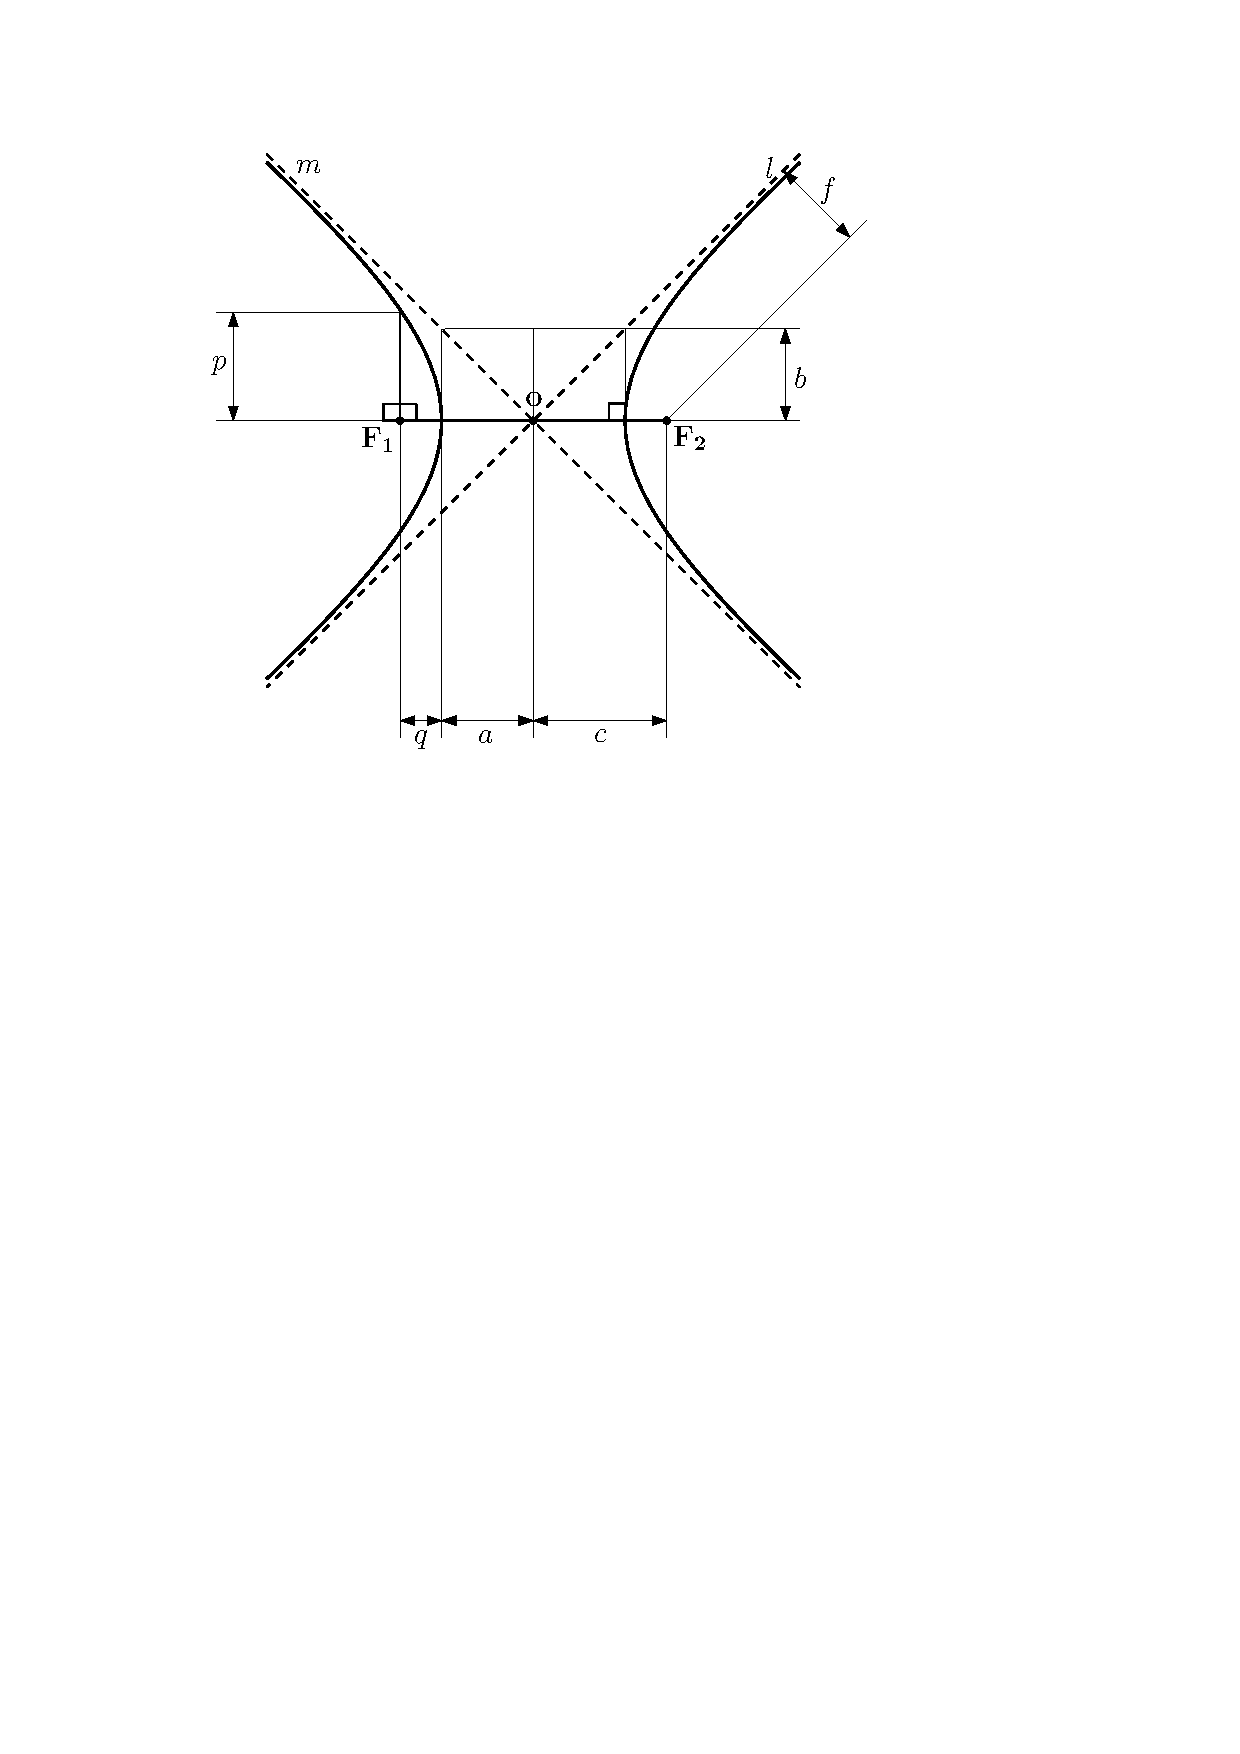
\includegraphics[width = 0.6\textwidth]{Hiperbola}
\caption{Гипербола \label{pic:the-pic}}
\end{figure}

Ближайшие друг к другу точки двух ветвей гиперболы называются \term{вершинами} гиперболы.

\term{Большая} или \term{действительная полуось} ($a$) гиперболы --- расстояние от центра гиперболы до одной из вершин.

\term{Действительная} или \term{поперечная} ось ---  прямая, содержащая большую ось гиперболы

\term{Фокальное расстояние} ($c$) ---  расстояние от центра гиперболы до одного из фокусов.

\term{Эксцентриситетом} гиперболы ($e$), как и  эллипса, является отношение фокального расстояния к большой полуоси, так как большая полуось гиперболы всегда больше ее фокального расстояния, эксцентриситет гиперболы $e > 1$ и может быть найдет из определения:\begin{equation}
e=\frac{c}{a}
\end{equation}

\term{Перицентрическое расстояние} ($q$) --- расстояние от фокуса до ближайшей вершины гиперболы.\begin{equation}
q=a(e-1)
\end{equation}

\term{Мнимая полуось} ($b$) --- длина перпендикуляра к оси абсцисс, восставленного из вершины до пересечения с асимптотой. Равна прицельному параметру.

\term{Мнимая} или \term{сопряжённая} ось --- прямая, перпендикулярная действительной оси и проходящая через её центр.

\term{Прицельный параметр} ($f$) --- расстояние от фокуса до асимптоты гиперболы.

\term{Фокальный параметр} ($p$) --- длина отрезка, перпендикулярного к действительной оси, проведённого от фокуса до гиперболы.
\begin{equation}
p=\frac{b^2}{a}
\end{equation}\\

Каноническое уравнение гиперболы в прямоугольных декартовых координатах записывается следующим образом:\begin{equation}
\frac{x^2}{a^2}-\frac{y^2}{b^2}=1
\end{equation}

В полярных координатах уравнение принимает следующий вид:\begin{equation}
r=\frac{p}{1-e\cos\varphi},
\end{equation}
причём полюс находится в фокусе гиперболы, а вершина гиперболы лежит на продолжении полярной оси.\\

Уравнение двух асимптот является уравнением пересекающихся прямых и принимает следующий вид:\begin{equation}
\frac{x}{a}\pm\frac{y}{b}=0
\end{equation}\\

Ниже представлены важные соотношения, справедливые для гиперболы:
\begin{equation}
c^2=a^2+b^2
\end{equation}\\

Также, как и любое коническое сечение, гипербола имеет своё оптическое свойство: свет от источника, находящегося в одном из фокусов гиперболы, отражается второй ветвью гиперболы таким образом, что продолжения отраженных лучей пересекаются во втором фокусе.
